\subsection{Motor model}


\subsubsection{d-direction}
\begin{figure}[H]
	\centering
	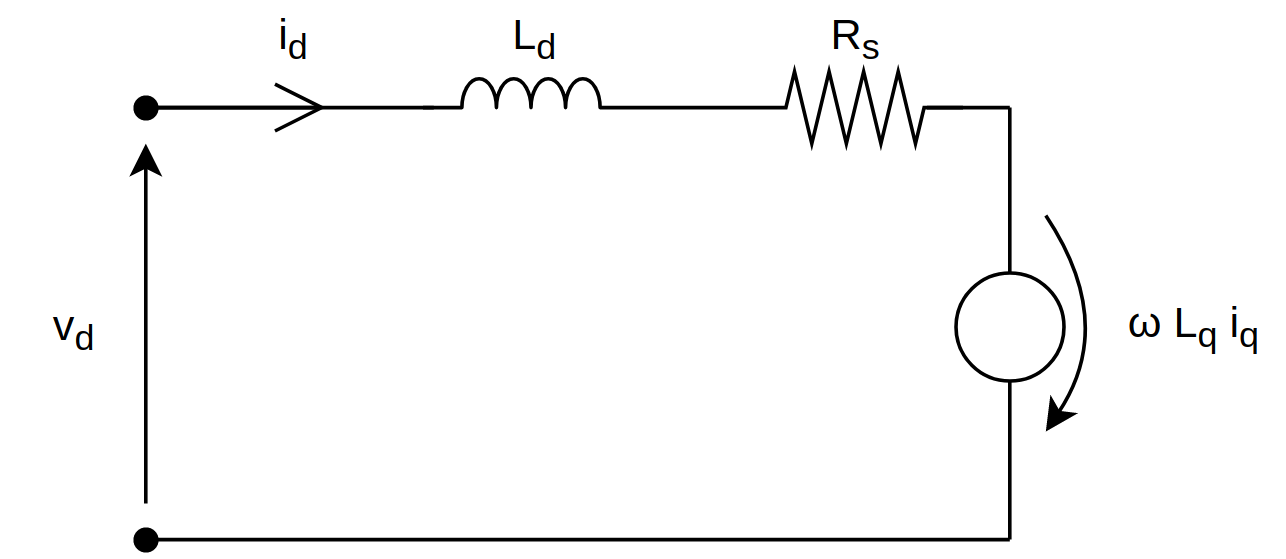
\includegraphics[width=0.6\linewidth]{pictures/control/vd}
	\caption{}
	\label{fig:vd}
\end{figure}


\begin{equation}\label{eq:d_direction}
v_d = L_d \frac{d i_d}{dt} + R_s i_d - \omega L_q i_q
\end{equation}
% $\varphi_{rq} = L_qi_q$
% \begin{equation}\label{eq:d_direction2}
% v_{d} = \frac{d \varphi_{rq}}{dt} + R_s i_d - \omega \varphi_{rq}
% \end{equation}


\begin{figure}[H]
	\centering
	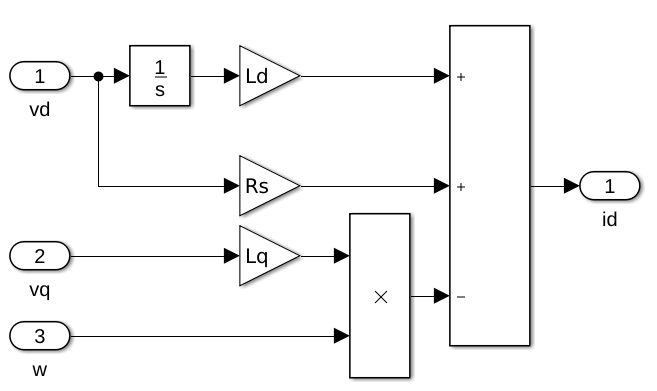
\includegraphics[width=0.6\linewidth]{pictures/control/simulink_d_direction.png}
	\caption{}
	\label{fig:simulink_d_direction}
\end{figure}



\subsubsection{q-direction}
\begin{figure}[H]
	\centering
	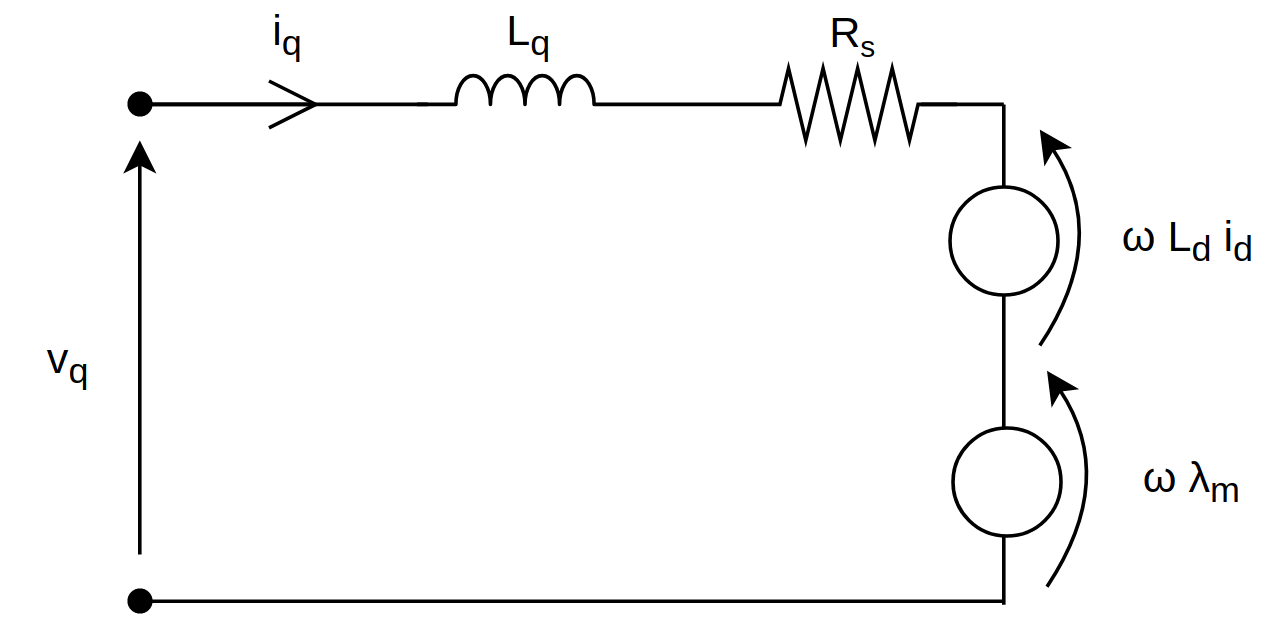
\includegraphics[width=0.6\linewidth]{pictures/control/vq.png}
	\caption{}
	\label{fig:vq}
\end{figure}
\begin{equation}\label{eq:q_direction}
v_q = L_q\frac{d i_q}{dt} + R_s i_q + \omega L_d i_d + \omega \lambda_m
\end{equation}

% \begin{equation}\label{eq:q_direction2}
% v_{sq} = R_si_q + \frac{d \varphi_{rd}}{dt} +  \omega_e \varphi_{rd}
% \end{equation}
% Where \\
% $\varphi_{rd} = L_di_d$

\begin{figure}[H]
	\centering
	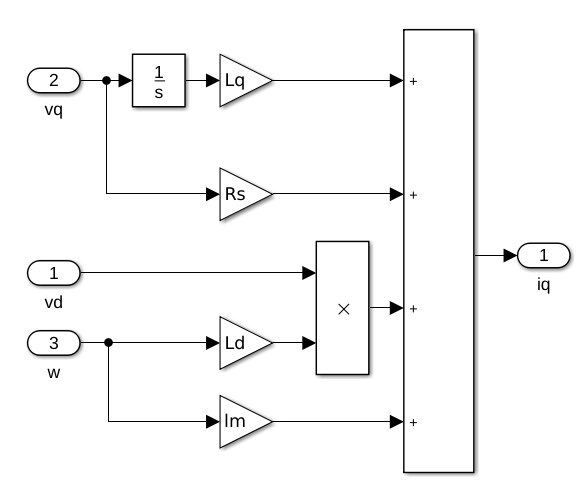
\includegraphics[width=0.5\linewidth]{pictures/control/simulink_q_direction.png}
	\caption{}
	\label{fig:simulink_d_direction}
\end{figure}

\subsubsection{Output torque}
For a multiple pole synchronous motor, the torque can be found from equation \ref{eq:torque_equation}.
\begin{equation}\label{eq:torque_equation}
T_e = \frac{3}{2} p (\Phi_{rd} i_{sq} - i_{sd} \Phi_{rq})
\end{equation}
Where $p$ is the number of poles.

As can be seen from the equation the current running in the d-direction produces negative torque and is therefore reducing the output torque. 
